\documentclass[14pt]{extbook}
\usepackage{multicol, enumerate, enumitem, hyperref, color, soul, setspace, parskip, fancyhdr} %General Packages
\usepackage{amssymb, amsthm, amsmath, bbm, latexsym, units, mathtools} %Math Packages
\everymath{\displaystyle} %All math in Display Style
% Packages with additional options
\usepackage[headsep=0.5cm,headheight=12pt, left=1 in,right= 1 in,top= 1 in,bottom= 1 in]{geometry}
\usepackage[usenames,dvipsnames]{xcolor}
\usepackage{dashrule}  % Package to use the command below to create lines between items
\newcommand{\litem}[1]{\item#1\hspace*{-1cm}\rule{\textwidth}{0.4pt}}
\pagestyle{fancy}
\lhead{Progress Quiz 5}
\chead{}
\rhead{Version B}
\lfoot{9912-2038}
\cfoot{}
\rfoot{Spring 2021}
\begin{document}

\begin{enumerate}
\litem{
Construct the lowest-degree polynomial given the zeros below. Then, choose the intervals that contain the coefficients of the polynomial in the form $ax^3+bx^2+cx+d$.\[ \frac{7}{2}, 2, \text{ and } \frac{1}{2} \]\begin{enumerate}[label=\Alph*.]
\item \( a \in [3, 5], b \in [0, 7], c \in [-32, -29], \text{ and } d \in [13, 21] \)
\item \( a \in [3, 5], b \in [-31, -17], c \in [36, 41], \text{ and } d \in [13, 21] \)
\item \( a \in [3, 5], b \in [-31, -17], c \in [36, 41], \text{ and } d \in [-19, -5] \)
\item \( a \in [3, 5], b \in [16, 21], c \in [16, 19], \text{ and } d \in [-19, -5] \)
\item \( a \in [3, 5], b \in [24, 25], c \in [36, 41], \text{ and } d \in [13, 21] \)

\end{enumerate} }
\litem{
Describe the zero behavior of the zero $x = 9$ of the polynomial below.\[ f(x) = -8(x + 2)^{7}(x - 2)^{4}(x + 9)^{8}(x - 9)^{7} \]\begin{enumerate}[label=\Alph*.]
\begin{multicols}{2}\item 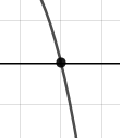
\includegraphics[width = 0.3\textwidth]{../Figures/polyZeroBehaviorAB.png}\item 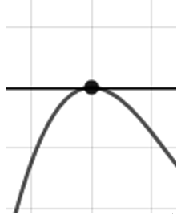
\includegraphics[width = 0.3\textwidth]{../Figures/polyZeroBehaviorBB.png}\item 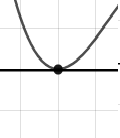
\includegraphics[width = 0.3\textwidth]{../Figures/polyZeroBehaviorCB.png}\item 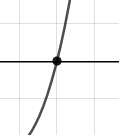
\includegraphics[width = 0.3\textwidth]{../Figures/polyZeroBehaviorDB.png}\end{multicols}\item None of the above.
\end{enumerate} }
\litem{
Describe the end behavior of the polynomial below.\[ f(x) = 8(x + 4)^{3}(x - 4)^{6}(x + 9)^{4}(x - 9)^{5} \]\begin{enumerate}[label=\Alph*.]
\begin{multicols}{2}\item 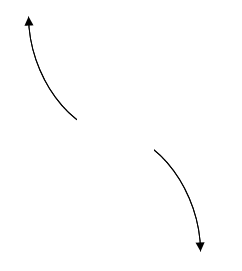
\includegraphics[width = 0.3\textwidth]{../Figures/polyEndBehaviorAB.png}\item 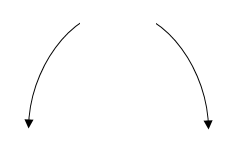
\includegraphics[width = 0.3\textwidth]{../Figures/polyEndBehaviorBB.png}\item 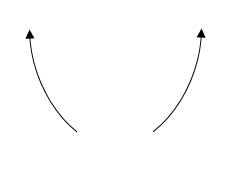
\includegraphics[width = 0.3\textwidth]{../Figures/polyEndBehaviorCB.png}\item 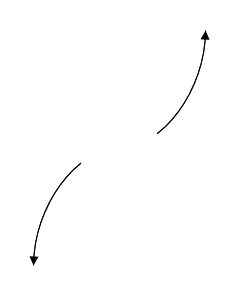
\includegraphics[width = 0.3\textwidth]{../Figures/polyEndBehaviorDB.png}\end{multicols}\item None of the above.
\end{enumerate} }
\litem{
Describe the zero behavior of the zero $x = 4$ of the polynomial below.\[ f(x) = 4(x + 2)^{5}(x - 2)^{4}(x + 4)^{5}(x - 4)^{4} \]\begin{enumerate}[label=\Alph*.]
\begin{multicols}{2}\item 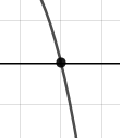
\includegraphics[width = 0.3\textwidth]{../Figures/polyZeroBehaviorCopyAB.png}\item 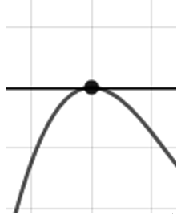
\includegraphics[width = 0.3\textwidth]{../Figures/polyZeroBehaviorCopyBB.png}\item 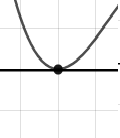
\includegraphics[width = 0.3\textwidth]{../Figures/polyZeroBehaviorCopyCB.png}\item 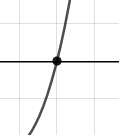
\includegraphics[width = 0.3\textwidth]{../Figures/polyZeroBehaviorCopyDB.png}\end{multicols}\item None of the above.
\end{enumerate} }
\litem{
Describe the end behavior of the polynomial below.\[ f(x) = 2(x + 3)^{4}(x - 3)^{9}(x + 9)^{4}(x - 9)^{5} \]\begin{enumerate}[label=\Alph*.]
\begin{multicols}{2}\item 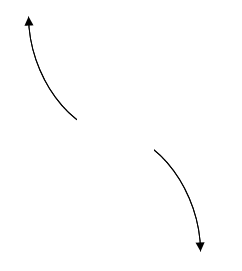
\includegraphics[width = 0.3\textwidth]{../Figures/polyEndBehaviorCopyAB.png}\item 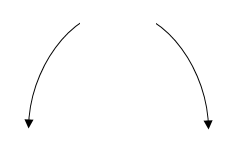
\includegraphics[width = 0.3\textwidth]{../Figures/polyEndBehaviorCopyBB.png}\item 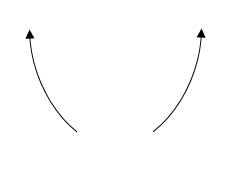
\includegraphics[width = 0.3\textwidth]{../Figures/polyEndBehaviorCopyCB.png}\item 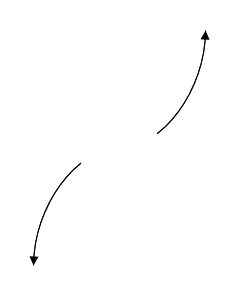
\includegraphics[width = 0.3\textwidth]{../Figures/polyEndBehaviorCopyDB.png}\end{multicols}\item None of the above.
\end{enumerate} }
\litem{
Construct the lowest-degree polynomial given the zeros below. Then, choose the intervals that contain the coefficients of the polynomial in the form $x^3+bx^2+cx+d$.\[ -4 - 5 i \text{ and } -4 \]\begin{enumerate}[label=\Alph*.]
\item \( b \in [6, 13], c \in [72.58, 73.76], \text{ and } d \in [162.4, 169] \)
\item \( b \in [-3, 10], c \in [8.81, 9.58], \text{ and } d \in [19.5, 21.2] \)
\item \( b \in [-3, 10], c \in [7.93, 8.59], \text{ and } d \in [15.7, 18.2] \)
\item \( b \in [-15, -4], c \in [72.58, 73.76], \text{ and } d \in [-165.5, -160.5] \)
\item \( \text{None of the above.} \)

\end{enumerate} }
\litem{
Construct the lowest-degree polynomial given the zeros below. Then, choose the intervals that contain the coefficients of the polynomial in the form $x^3+bx^2+cx+d$.\[ -3 + 5 i \text{ and } -4 \]\begin{enumerate}[label=\Alph*.]
\item \( b \in [-12, -7], c \in [50, 59], \text{ and } d \in [-140, -131] \)
\item \( b \in [5, 18], c \in [50, 59], \text{ and } d \in [136, 142] \)
\item \( b \in [-3, 9], c \in [-5, 5], \text{ and } d \in [-26, -19] \)
\item \( b \in [-3, 9], c \in [2, 14], \text{ and } d \in [7, 17] \)
\item \( \text{None of the above.} \)

\end{enumerate} }
\litem{
Which of the following equations \textit{could} be of the graph presented below?
\begin{center}
    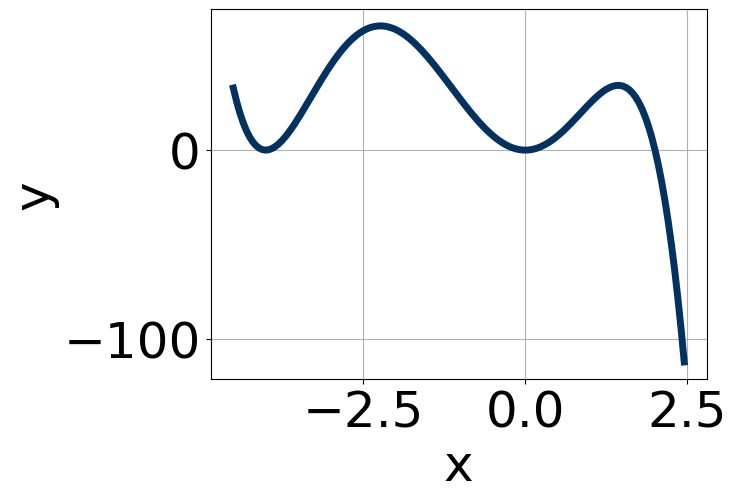
\includegraphics[width=0.5\textwidth]{../Figures/polyGraphToFunctionCopyB.png}
\end{center}
\begin{enumerate}[label=\Alph*.]
\item \( 4(x + 3)^{4} (x + 1)^{4} (x - 2)^{11} \)
\item \( 18(x + 3)^{4} (x + 1)^{9} (x - 2)^{7} \)
\item \( -15(x + 3)^{8} (x + 1)^{9} (x - 2)^{7} \)
\item \( -19(x + 3)^{7} (x + 1)^{5} (x - 2)^{11} \)
\item \( 13(x + 3)^{7} (x + 1)^{5} (x - 2)^{7} \)

\end{enumerate} }
\litem{
Construct the lowest-degree polynomial given the zeros below. Then, choose the intervals that contain the coefficients of the polynomial in the form $ax^3+bx^2+cx+d$.\[ \frac{-7}{5}, \frac{-5}{3}, \text{ and } \frac{3}{4} \]\begin{enumerate}[label=\Alph*.]
\item \( a \in [60, 61], b \in [135, 149], c \in [-4, 9], \text{ and } d \in [-115, -100] \)
\item \( a \in [60, 61], b \in [-229, -223], c \in [275, 281], \text{ and } d \in [-115, -100] \)
\item \( a \in [60, 61], b \in [135, 149], c \in [-4, 9], \text{ and } d \in [104, 108] \)
\item \( a \in [60, 61], b \in [-32, -25], c \in [-153, -151], \text{ and } d \in [104, 108] \)
\item \( a \in [60, 61], b \in [-142, -136], c \in [-4, 9], \text{ and } d \in [104, 108] \)

\end{enumerate} }
\litem{
Which of the following equations \textit{could} be of the graph presented below?
\begin{center}
    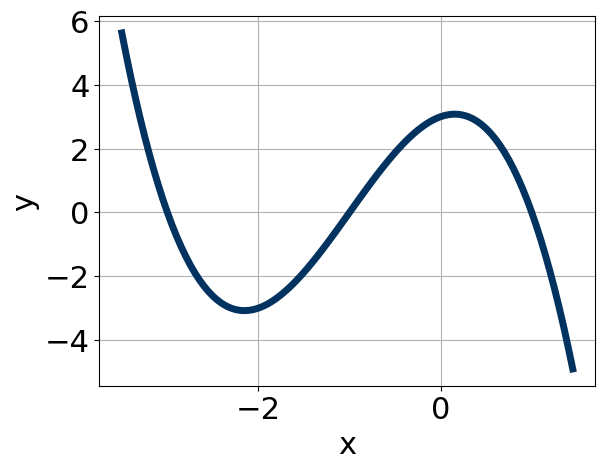
\includegraphics[width=0.5\textwidth]{../Figures/polyGraphToFunctionB.png}
\end{center}
\begin{enumerate}[label=\Alph*.]
\item \( -5(x + 2)^{4} (x - 2)^{5} (x + 1)^{5} \)
\item \( 8(x + 2)^{7} (x - 2)^{9} (x + 1)^{7} \)
\item \( 17(x + 2)^{4} (x - 2)^{10} (x + 1)^{11} \)
\item \( 18(x + 2)^{8} (x - 2)^{9} (x + 1)^{9} \)
\item \( -16(x + 2)^{7} (x - 2)^{11} (x + 1)^{7} \)

\end{enumerate} }
\end{enumerate}

\end{document}